\documentclass[12pt]{article}

\usepackage[utf8]{inputenc}
\usepackage{geometry}
\geometry{a4paper, margin=1in}
\usepackage{graphicx}
\usepackage{amsmath}
\usepackage{amssymb}
\usepackage{booktabs}
\usepackage{hyperref}
\usepackage{caption}

\title{\textbf{Machine Learning Assignment 1: Polynomial Regression Analysis}}
\author{Roll Number: IMT2024045}
\date{\today}

\begin{document}

\maketitle

\section{Introduction}
This report details the implementation and evaluation of a polynomial regression model developed entirely from scratch using NumPy. The objective is to predict the continuous target variable $y$ for two distinct scenarios: Steam Turbine Optimization (var1) and Subterranean Thermal Reservoir Mapping (var2). The report discusses the mathematical foundations aligned with the course notation, feature selection methodologies, and the determination of the optimal polynomial degree through hyperparameter sweeping using both standard hold-out and $K$-Fold cross-validation.

\section{Methodology and Mathematical Formulation}
Following the notation established in the lectures, let the $n^{\text{th}}$ data point be denoted by the input vector $\mathbf{x}_n$ and the true target value as $y_n$ (often denoted $t_n$ in standard literature). The predictor or hypothesis function is parameterized by weights $\mathbf{w}$ and is defined as:
\begin{equation}
f(\mathbf{x}_n; \mathbf{w}) = \mathbf{w}^T \mathbf{x}_n
\end{equation}

For polynomial regression of degree $d$ with $D$ original features, we expand the input vector $\mathbf{x}_n$ to include all combinations of polynomial terms (monomials) up to degree $d$. 

The model is optimized by minimizing the averaged Squared Loss function $\mathcal{L}$ over all $N$ data points:
\begin{equation}
\mathcal{L}(\mathbf{w}) = \frac{1}{N} \sum_{n=1}^{N} \mathcal{L}_n(y_n, f(\mathbf{x}_n; \mathbf{w})) = \frac{1}{N} \sum_{n=1}^{N} (y_n - \mathbf{w}^T \mathbf{x}_n)^2
\end{equation}

Let $\mathbf{X}$ be the data matrix where the $n^{\text{th}}$ row is $\mathbf{x}_n^T$, and let $\mathbf{y}$ be the column vector of targets. Setting the gradient of $\mathcal{L}(\mathbf{w})$ with respect to $\mathbf{w}$ to zero yields the Normal Equation:
\begin{equation}
\mathbf{X}^T \mathbf{X} \mathbf{w} = \mathbf{X}^T \mathbf{y}
\end{equation}

Solving for $\mathbf{w}$, we obtain the closed-form optimal weights:
\begin{equation}
\mathbf{w} = (\mathbf{X}^T \mathbf{X})^{-1} \mathbf{X}^T \mathbf{y}
\end{equation}

To ensure numerical stability when $\mathbf{X}^T \mathbf{X}$ is ill-conditioned (which is common in high-degree polynomial expansions), the implementation calculates the least-squares solution using Singular Value Decomposition via NumPy.

\section{Problem 1: Steam Turbine Optimization (var1)}
\subsection{Experimental Setup}
The objective is to predict the Net Power Score ($y$) based on 6 operational parameters ($x_1, \dots, x_6$). We performed two exhaustive sweeps across all subsets of features and polynomial degrees (from 1 to 10): first using a standard 80/20 train-validation split, and subsequently using a rigorous 10-Fold Cross-Validation to assess model stability.

\subsection{80/20 Split Analysis}
\begin{figure}[h]
    \centering
    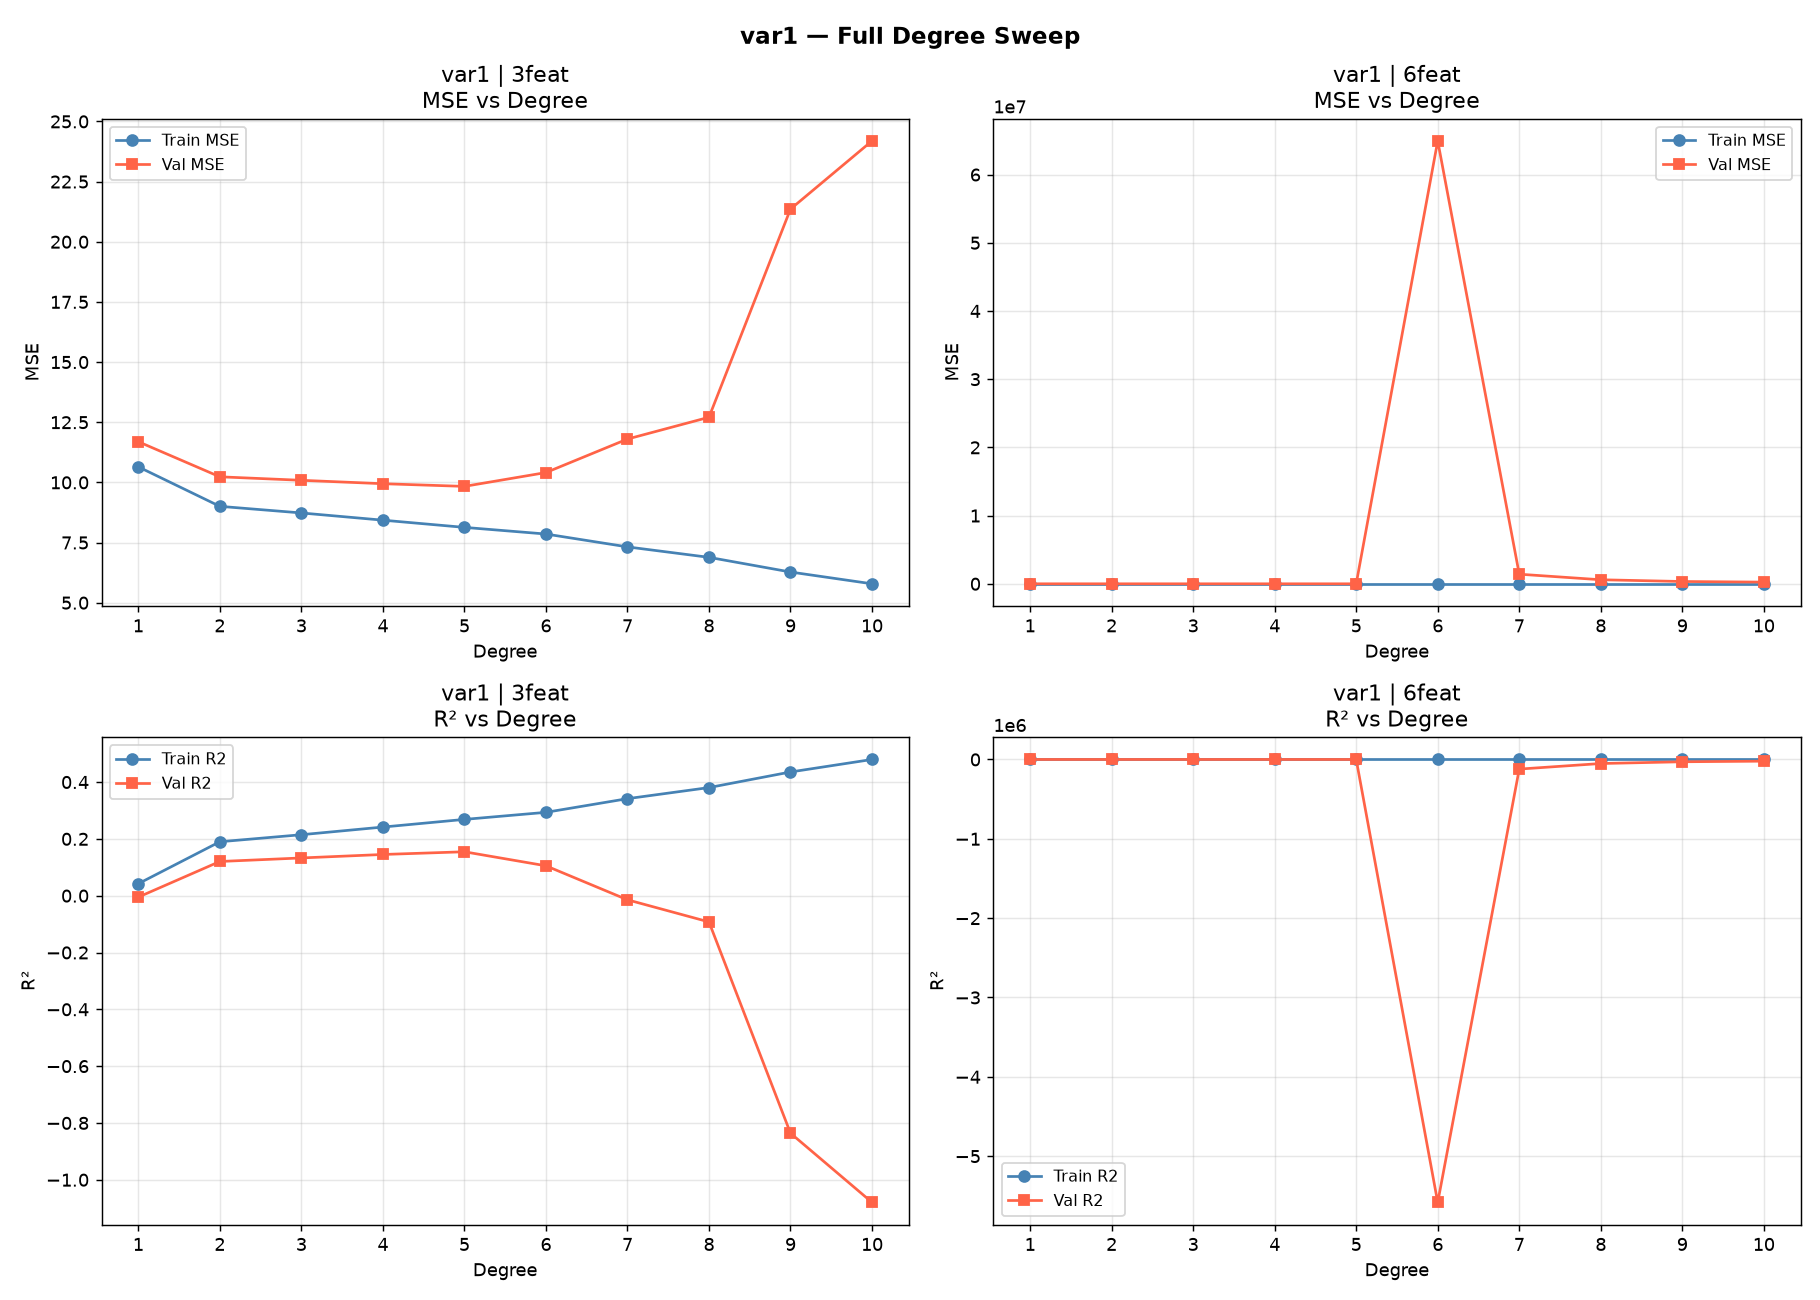
\includegraphics[width=0.9\textwidth]{var1_sweep.png}
    \caption{Degree Sweep for Problem 1 comparing different feature subsets (80/20 Split).}
    \label{fig:var1_sweep}
\end{figure}

\begin{table}[h]
\centering
\begin{tabular}{c c c | c c}
\toprule
\textbf{Degree} & \textbf{3 Features ($x_1, x_2, x_3$)} & & \textbf{6 Features ($x_1 \dots x_6$)} & \\
& Val MSE & Val $R^2$ & Val MSE & Val $R^2$ \\
\midrule
2 & 10.23 & 0.120 & 3.46 & 0.703 \\
3 & 10.09 & 0.133 & 1.12 & 0.904 \\
\textbf{4} & 9.95 & 0.145 & \textbf{0.835} & \textbf{0.928} \\
5 & 9.83 & 0.155 & 1.21 & 0.896 \\
6 & 10.41 & 0.105 & $6.49 \times 10^7$ & Explodes \\
\bottomrule
\end{tabular}
\caption{Validation performance across polynomial degrees (80/20 split) for Problem 1.}
\label{tab:var1_sweep}
\end{table}

As illustrated in Figure \ref{fig:var1_sweep} and Table \ref{tab:var1_sweep}, omitting features (e.g., using only 3 features) results in severe underfitting. Incorporating all 6 features yields an optimal validation MSE at \textbf{Degree 4} (MSE = 0.835). At Degree 6, the model suffers from extreme overfitting due to the curse of dimensionality.

\subsection{10-Fold Cross Validation Analysis}
To robustly verify this hyperparameter selection, a 10-Fold CV was applied to all 630 configurations (63 feature subsets $\times$ 10 degrees). The standard deviation of the validation MSE across the 10 folds was recorded as a metric of model stability.

\begin{table}[h]
\centering
\begin{tabular}{l c c c c}
\toprule
\textbf{Features Included} & \textbf{Degree} & \textbf{Avg Val MSE} & \textbf{Avg Val $R^2$} & \textbf{Val MSE Std Dev} \\
\midrule
$x_1, x_2, x_3, x_4, x_5, x_6$ & 3 & 1.108 & 0.901 & 0.235 \\
$\mathbf{x_1, x_2, x_3, x_4, x_5, x_6}$ & \textbf{4} & \textbf{0.833} & \textbf{0.924} & \textbf{0.144} \\
$x_1, x_2, x_3, x_4, x_5, x_6$ & 5 & 1.014 & 0.911 & 0.347 \\
$x_1, x_2, x_3, x_5, x_6$ (No $x_4$) & 4 & 1.753 & 0.841 & 0.224 \\
\bottomrule
\end{tabular}
\caption{Top configurations from 10-Fold Cross-Validation for Problem 1.}
\label{tab:var1_kfold}
\end{table}

The 10-Fold CV (Table \ref{tab:var1_kfold}) definitively confirms that \textbf{Degree 4 with all 6 features} is superior. Not only does it hold the lowest average error (MSE = 0.833), but it is also the most stable configuration, exhibiting the lowest variance across folds (Std Dev = 0.144).

\begin{figure}[h]
    \centering
    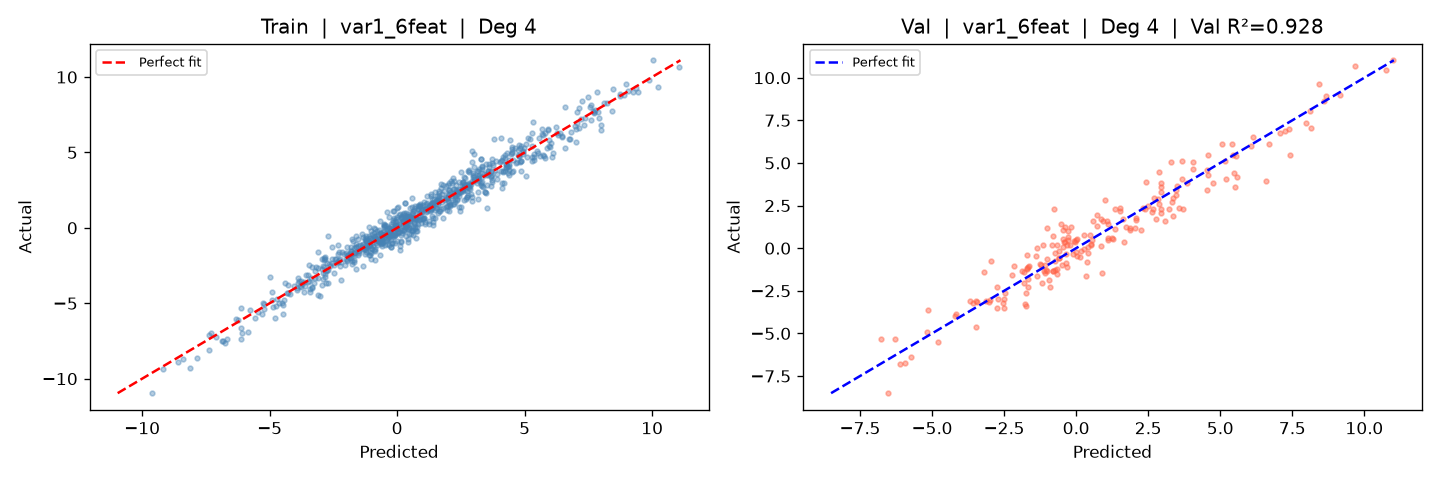
\includegraphics[width=0.85\textwidth]{var1_residuals.png}
    \caption{Residual Analysis for the optimal Degree 4 model (6 features).}
    \label{fig:var1_res}
\end{figure}

\section{Problem 2: Subterranean Thermal Reservoir Mapping (var2)}
\subsection{Experimental Setup}
The objective is to predict the Thermal Anomaly Score ($y$) using 3 spatial coordinate offsets ($x_1, x_2, x_3$). As with Problem 1, we evaluated models using both an 80/20 split and exhaustive 10-Fold CV across all possible 70 feature/degree permutations.

\subsection{80/20 Split Analysis}

\begin{figure}[h]
    \centering
    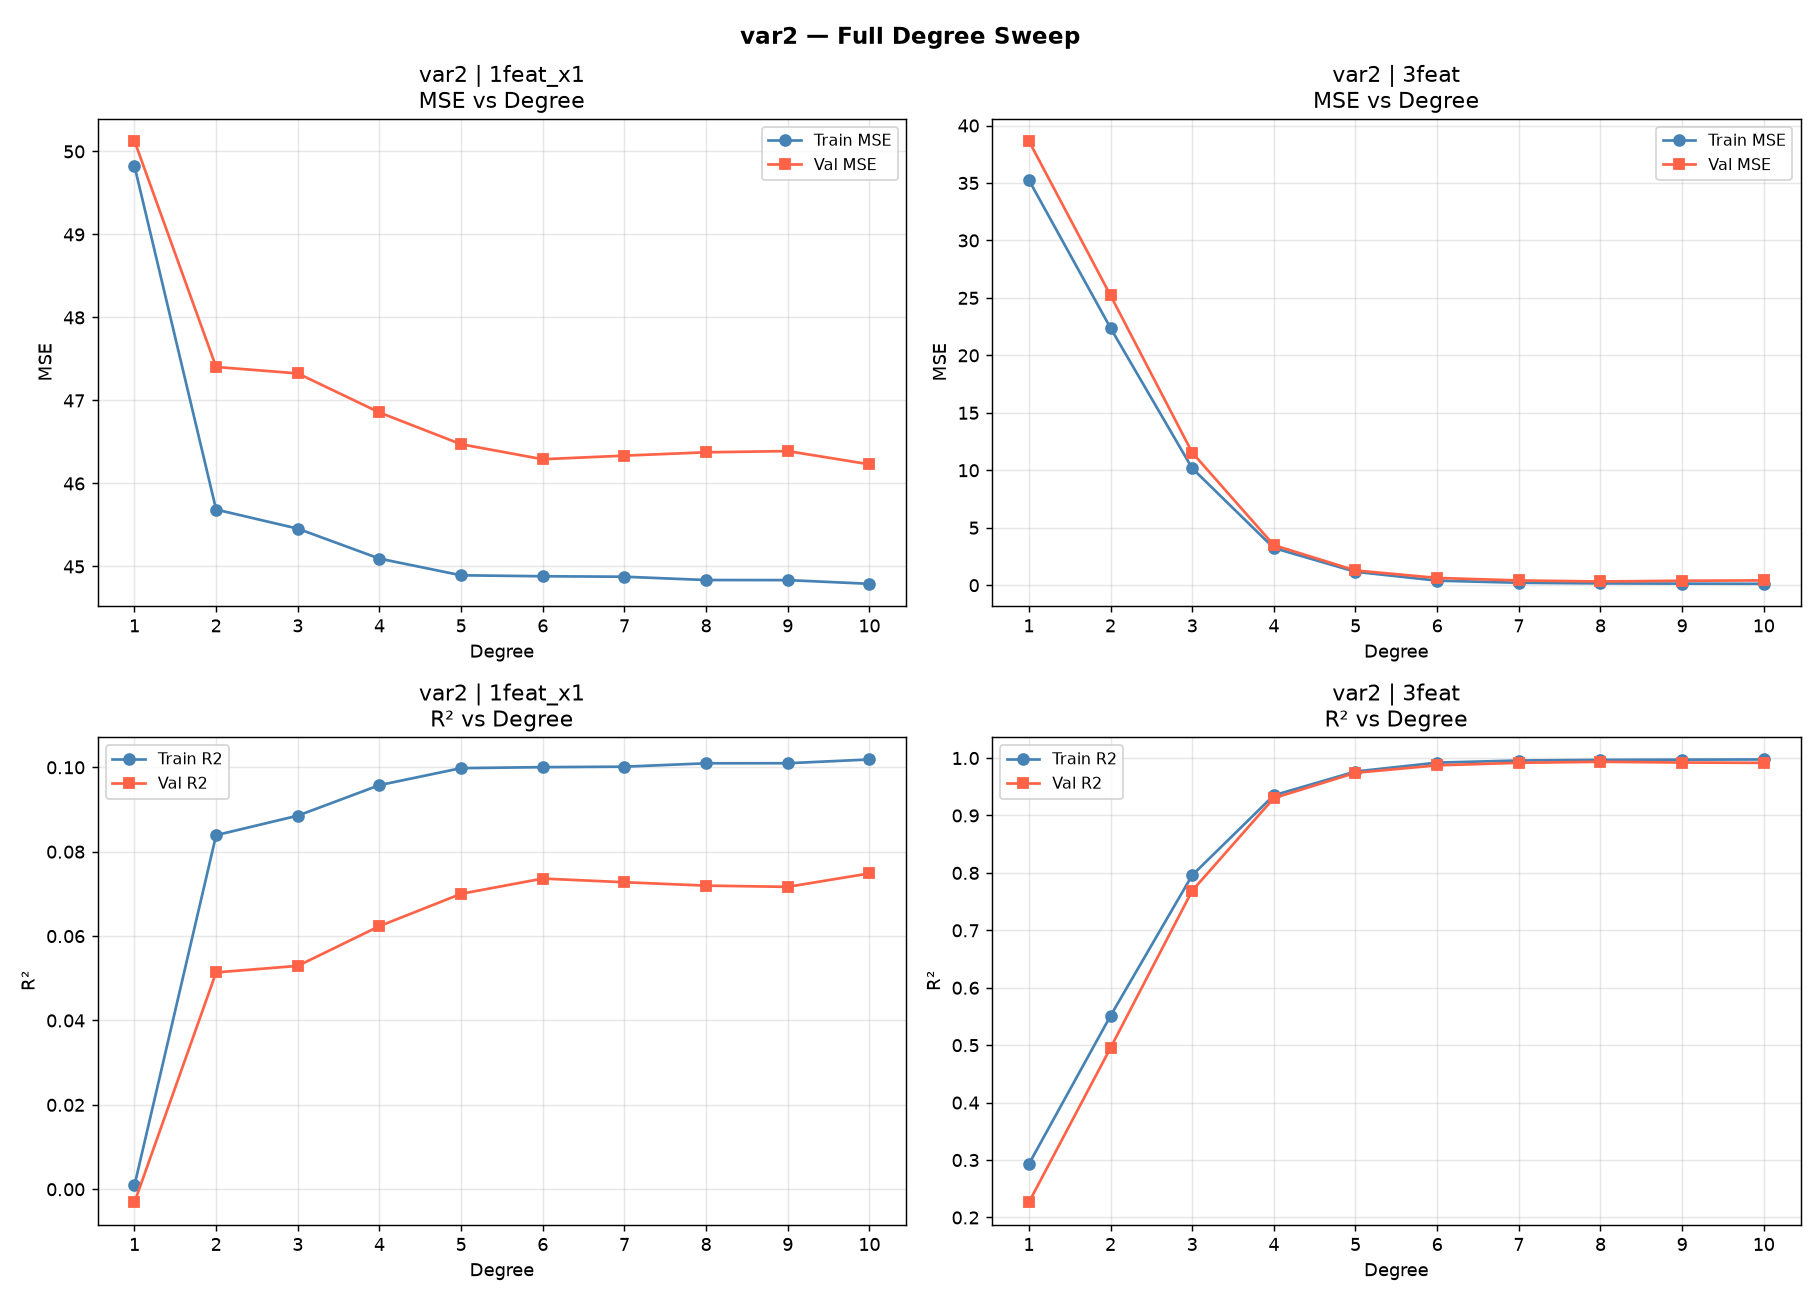
\includegraphics[width=0.9\textwidth]{var2_sweep.png}
    \caption{Degree Sweep for Problem 2 comparing different feature subsets.}
    \label{fig:var2_sweep}
\end{figure}

\begin{table}[h]
\centering
\begin{tabular}{c c c | c c}
\toprule
\textbf{Degree} & \textbf{1 Feature ($x_1$)} & & \textbf{3 Features ($x_1, x_2, x_3$)} & \\
& Val MSE & Val $R^2$ & Val MSE & Val $R^2$ \\
\midrule
4 & 46.86 & 0.062 & 3.48 & 0.930 \\
6 & 46.29 & 0.074 & 0.633 & 0.987 \\
\textbf{8} & 46.38 & 0.072 & \textbf{0.324} & \textbf{0.993} \\
10 & 46.23 & 0.075 & 0.416 & 0.992 \\
\bottomrule
\end{tabular}
\caption{Validation performance across polynomial degrees (80/20 split) for Problem 2.}
\label{tab:var2_sweep}
\end{table}

The initial 80/20 sweep (Figure \ref{fig:var2_sweep} and Table \ref{tab:var2_sweep}) reveals that using a single feature completely fails to capture the target variance. With 3 features, the model steadily improves, minimizing validation error at \textbf{Degree 8}.

\subsection{10-Fold Cross Validation Analysis}

\begin{table}[h]
\centering
\begin{tabular}{l c c c c}
\toprule
\textbf{Features Included} & \textbf{Degree} & \textbf{Avg Val MSE} & \textbf{Avg Val $R^2$} & \textbf{Val MSE Std Dev} \\
\midrule
$x_1, x_2, x_3$ & 6 & 0.573 & 0.988 & 0.069 \\
$x_1, x_2, x_3$ & 7 & 0.336 & 0.993 & 0.045 \\
$\mathbf{x_1, x_2, x_3}$ & \textbf{8} & \textbf{0.273} & \textbf{0.994} & \textbf{0.027} \\
$x_1, x_2, x_3$ & 9 & 0.297 & 0.994 & 0.028 \\
$x_1, x_2, x_3$ & 10 & 0.401 & 0.992 & 0.196 \\
\bottomrule
\end{tabular}
\caption{Top configurations from 10-Fold Cross-Validation for Problem 2.}
\label{tab:var2_kfold}
\end{table}

The 10-Fold CV results in Table \ref{tab:var2_kfold} corroborate the 80/20 findings. At \textbf{Degree 8}, the validation MSE achieves its true minimum (0.273) alongside an exceptional stability metric (Std Dev = 0.027). Pushing the polynomial to Degree 10 drastically increases the standard deviation (0.196), indicating the onset of model variance.

\begin{figure}[h]
    \centering
    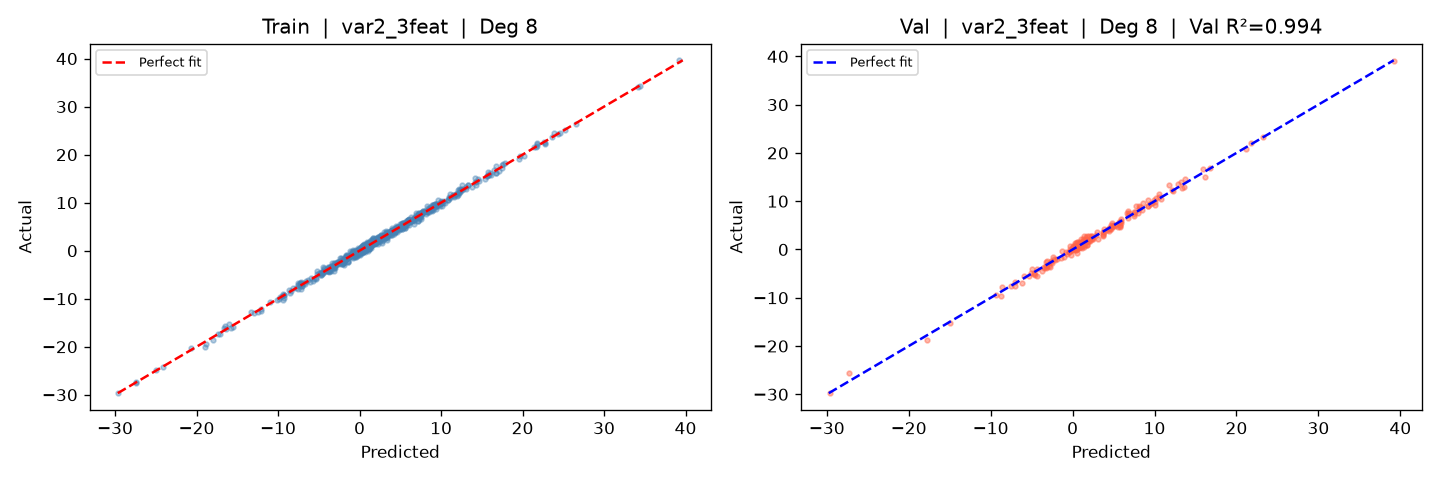
\includegraphics[width=0.85\textwidth]{var2_residuals.png}
    \caption{Residual Analysis for the optimal Degree 8 model (3 features).}
    \label{fig:var2_res}
\end{figure}

The residual plot in Figure \ref{fig:var2_res} confirms that the validation predictions tightly hug the perfect-fit line. Consequently, the \textbf{Degree 8 model with all 3 features} was definitively chosen as the final model for Problem 2.

\section{Conclusion}
Through systematic feature selection and hyperparameter sweeping via both 80/20 splits and rigorous 10-Fold Cross-Validation, optimal polynomial regression models were mathematically identified. The analysis demonstrated that leveraging the full feature set up to an optimal complexity boundary accurately minimizes the squared loss $\mathcal{L}(\mathbf{w})$ while maintaining model stability across holdout folds.

\end{document}
